%%%%%%%%%%%%%%%%%%
% Ch1 : Architecture atomique %
%%%%%%%%%%%%%%%%%%

\chapter{Architecture atomique}
\section{Atome : fiche technique}
\noindent Commençons par un bref rappel des propriétés principales : \\
\begin{itemize}
	\item[•] Le noyeau est formé de \textbf{protons} et \textbf{neutrons}, appelés \textbf{nucléons} et entouré d'\textbf{électrons} qui se déplacent dans des \textbf{orbitales} dictées par la fonction d'onde.
	\item[•] Le \textbf{nombre atomique Z} désigne le nombre d'électrons = le nombre de protons. 
	\item[•] Le nombre de neutrons peut différer pour un même atome donnant lieu à des \textbf{isotopes}.
	\item[•] La masse d'un nucléon est de $\mathbf{1.66 \, 10^{-24} \,g}$ et celle de l'électron de $\mathbf{9.1 \, 10^{-31} \,g}$ (rapport 1/1800).
	\item[•] La charge d'un électron est de $\mathbf{1.602 \, 10^{-19} \, g}$.
	\item[•] L'unité de \textbf{mole} correspond à $\mathbf{6.02 \, 10^{23}}$ \textbf{particules} (nombre d'avogadro) et une mole de nucléons pèse $\mathbf{1\, g}$.
\end{itemize}
	
\section{Comportement ondulatoire de l'électron}

\subsection{Dualité onde/corpuscule}
\noindent Etudié en long et en large dans le cours de \emph{Physique quantique II}, on sait grâce à \textbf{de Broglie} qu'une onde est associée à toute particule et sa longueur d'onde est donnée par 
\begin{equation}
	\lambda = \frac{h}{p} = \frac{h}{mv} \qquad \mathbf{h = 6.62 \, 10^{-34} \, J.s} \mbox{ (contante de Planck)}	
\end{equation}
\noindent En 1927, Davisson et Germer mettent en évidence expérimentalement cet aspect grâce au phénomène d'\textbf{interférence}. \\
En 1926, \textbf{Schrödinger} proposera que l'onde associée à un électron en mouvement résulte de la variation périodique d'une fonction $\psi$ appelée \textbf{fonction d'onde}. Les électrons seront alors dans des orbitales occupant un volume de l'espace et non plus dans des orbites circulaires.  
	
\noindent De plus, les états énergétiques correspondent à des ondes stationnaires qu'on peut caractériser par l'équation 
\begin{equation}
	\frac{d^2}{dx^2}a + \frac{4\pi ^2}{\lambda ^2}a = 0
	\label{equation:1.2}
\end{equation}	 
qui régit également les oscillations d'une corde fixée à ses deux extrémités, à une dimension. L'amplitude $a$ varie en fonction de la position $x$ sur la corde pour un $\lambda$ donné. \\
En se rappelant que $E_{cin} = E-V = \frac{1}{2}mv^2$ et en remplaçant l'amplitude de \eqref{equation:1.2} par $\psi$, on retrouve l'équation de Schrödinger à une dimension 
\begin{equation}
	-\frac{\hbar ^2}{2m}\frac{d^2}{dx^2}\psi = (E-V)\psi
\end{equation}
Rappelons-nous qu'on obtient la \textbf{probabilité de présence} avec $\int |\psi| ^2 \, dV.$
	
\subsection{Orbitales et nombres quantiques}
\noindent On sait donc que chaque atome possède un certain nombre d'orbitales électroniques caractérisées par des valeurs de l'énergie. Seules les orbitales de plus \textbf{basses énergies} sont occupées. Ces dernières sont définies par 4 nombres quantique :\\
\begin{itemize}
	\item[•] \textbf{Le nombre quantique principal n} $(n>0)$ qui fixe la \textbf{taille} de l'orbital. On associe les lettres K, L, M,\dots \ à $n=1,2,3, \dots$
	\item[•] \textbf{Le nombe quantique azimutal l} $(0<l<n-1)$ qui fixe la forme de l'orbitale. Les sous-niveaux énergétique $l = 0,1,2, \dots$ sont désingnés par les lettres s (sphérique), p, d, f,\dots
	\item[•] \textbf{Le nombre quantique magnétique } $\mathbf{m_l}$ $(-l <m_l<l)$ qui fixe l'orientation de l'orbitale. 
	\item[•] \textbf{Le nombre quantique de spin} $\mathbf{ m_s}$ $(1/2$ ou $-1/2)$ qui ne décrit en rien l'orbital mais correspond au sens de la rotation de l'électron. \\
\end{itemize}
On dit que $n$ définit la couche, $l$ la sous-couche et $m_l$ définit la case quantique où on trouve maximum 2 électrons selon le \textbf{principe de Pauli} qui dit que 2 électrons d'un même atome ne peuvent avoir les 4 mêmes nombres quantiques. 
	
\subsection{Formes des orbitales}
\begin{wrapfigure}[4]{l}{4.7cm}
	\vspace{-5mm}
	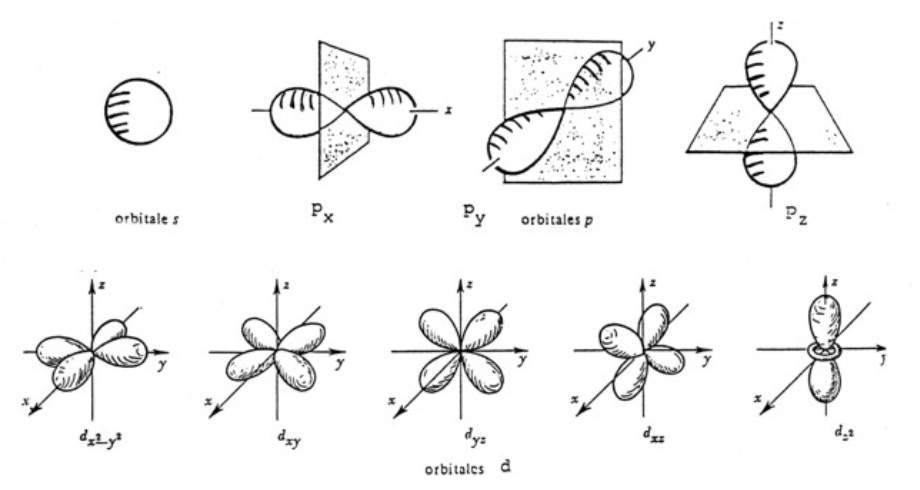
\includegraphics[scale=0.3]{ch1/1}
\end{wrapfigure}
Ces orbitales doivent être interprétés comme des domaines de haute probabilité de présence de l'électron. C'est $l$ qui détermine la forme et on sait que les orbitales $s\, (l=0)$ sont sphériques. Les autres sont plus complexe. \\
		
\subsection{Règle régissant le remplissage des électrons}
\subsubsection{Principe de Pauli}
Le \textbf{principe de Pauli} indique que si 2 électrons sont dans une même case quantique, alors ils ont des \textbf{spins opposés}, impliquant directement la \textbf{règle de Stoner} : le nombre maximum d'électrons sur une couche est de $2n^2$. 
	
\subsubsection{Règle de Klechkovsky}
La \textbf{règle de Klechkovsky} dit que la distribution des électrons se fait selon l'ordre des énergies des orbitales en commençant par la plus faible. Pour un atome \textbf{monoélectronique}, cette énergie croît avec $n$ alors que pour les \textbf{polyélectroniques}, elle est lié à $n+l$. Pour une même valeur de $n+l$, l'énergie la plus faible se retrouve pour le plus petit $n$. Cette règle est la raison pour laquelle la couche $4s$ se remplit avant la $3d$ qui est plus proche du noyau.\\
	
\subsubsection{Principe de Hund}
\begin{wrapfigure}[5]{r}{4.7cm}
	\vspace{-5mm}
	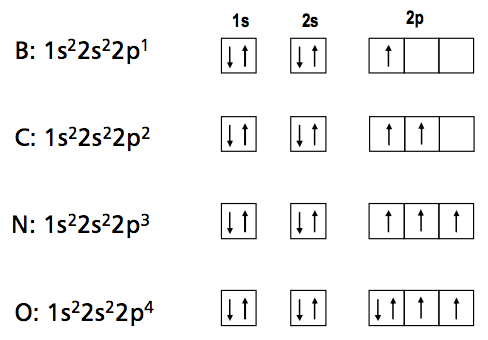
\includegraphics[scale=0.6]{ch1/2}
\end{wrapfigure}
Lorsqu'il y a possibilité d'utiliser plusieurs orbitales de même énergie au sein d'une sous-couche, l'état d'énergie atomique minimale est celui obtenu par l'occupation d'un maximum de cases quantiques. Les électrons tendent donc à s'éloigner et à rester célibataires. Ces électrons sont à la base des propriétés magnétiques des matériaux. 
	
\section{Tableau de Mendeleiev}
\begin{wrapfigure}[11]{l}{6.7cm}
	\vspace{-5mm}
	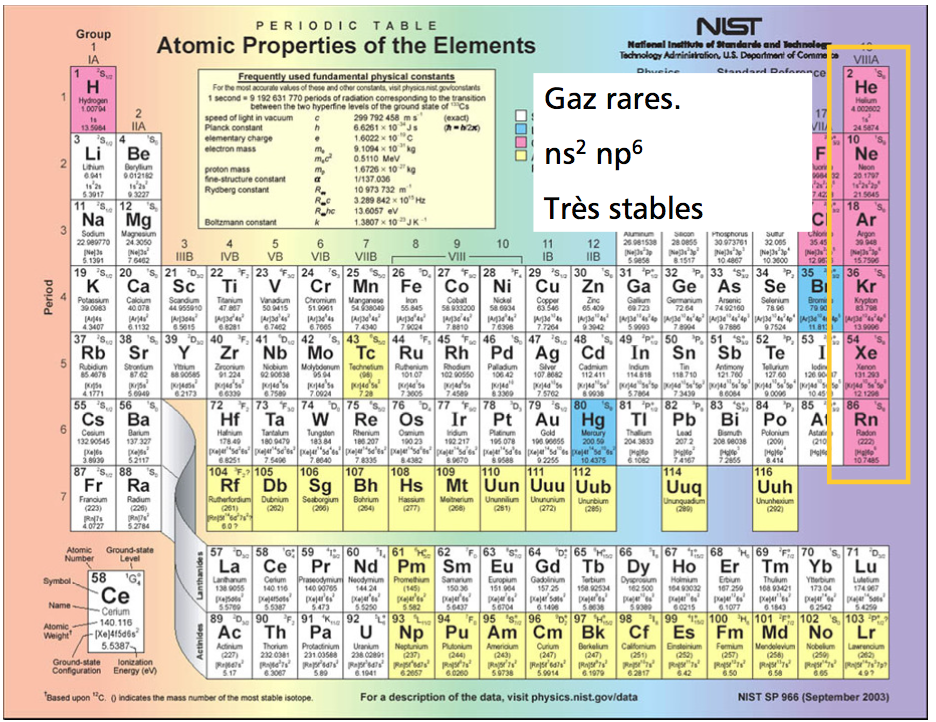
\includegraphics[scale=0.4]{ch1/3}
\end{wrapfigure}
On sait tous ce que c'est. Rappelons que les éléments dans une même colonne forment un groupe et ont des propriétés chimiques comparables (ex : la valence). Au départ, la place des éléments suivaient l'évolution de la masse atomique des éléments, alors que, maintenant, elle suit le nombre atomique (remplissage des couches).\\
La configuration de la dernière couche dans une même colonne est la même. Ainsi, les éléments de la dernière colonne (les gaz rares) ont une couche externe comportant 8 électrons, les rendant très stables. L'ajout d'un électron se fait sur la couche suivante. C'est pour ça qu'ils sont très peu réactifs (atomes isolés). \\
La première colonne du tableau contient les alcalins. Ils ne possèdent qu'un électron sur leur couche de valence et suivent directement les gaz rares. La perte de cet électron par oxydation les fait revenir à la configuration de gaz rare. Les autres éléments du tableau suivent le même raisonnement. Il faut juste faire attention que certains éléments peuvent revenir non seulement à l'état du gaz rare suivant mais aussi à celui du gaz rare qui les précède. \\
	
\begin{wrapfigure}[9]{r}{6.6cm}
	\vspace{-5mm}
	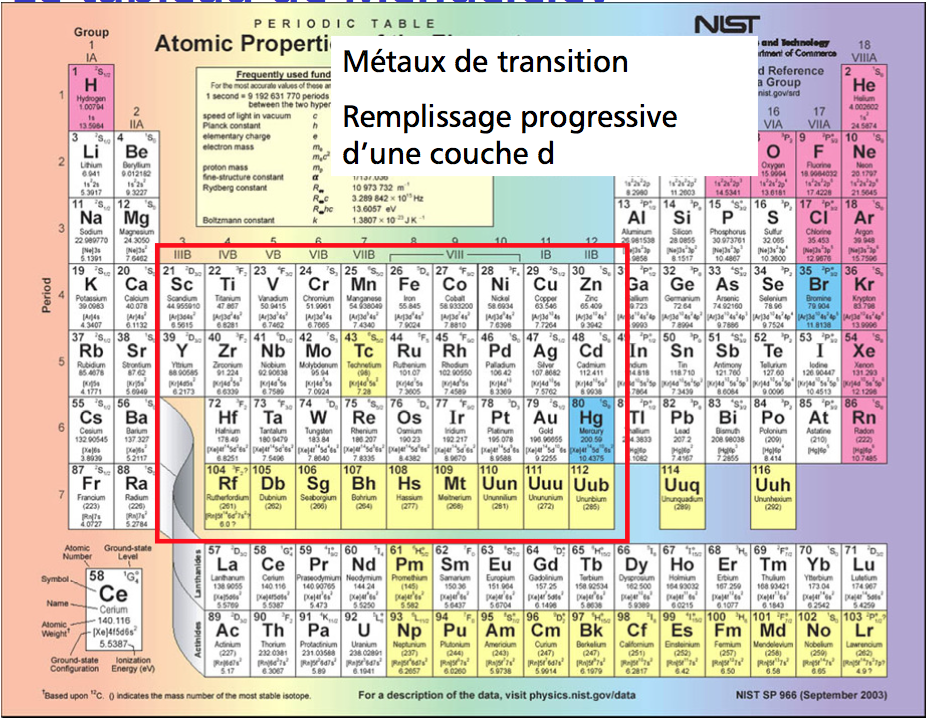
\includegraphics[scale=0.4]{ch1/4}
\end{wrapfigure}
La majeure partie des éléments sont des métaux. Les non-métaux se retrouvent à droite. Le milieu du tableau est occupé par les éléments de transition. Le remplissage des orbitales $(n+1) \, s$ précède toujours celle des $nd$. L'existence d'un niveau partiellement occupé va procurer des propriétés particulières à ces éléments.
	
	
	
	